\documentclass[aspectratio=169,10pt]{beamer}

% ── Theme & Styling ───────────────────────────────────────────────────────────
\usetheme{Madrid}
\usecolortheme{whale}

% ── NITK Colors ───────────────────────────────────────────────────────────────
\definecolor{nitkblue}{rgb}{0.0,0.14,0.38}
\definecolor{accentblue}{rgb}{0.0,0.45,0.81}
\definecolor{darkslate}{rgb}{0.12,0.16,0.23}
\definecolor{cardbg}{rgb}{0.95,0.96,0.98}
\definecolor{successgreen}{rgb}{0.06,0.58,0.29}
\definecolor{alertred}{rgb}{0.82,0.15,0.15}

\setbeamercolor{palette primary}{bg=nitkblue,fg=white}
\setbeamercolor{palette secondary}{bg=accentblue,fg=white}
\setbeamercolor{palette tertiary}{bg=nitkblue,fg=white}
\setbeamercolor{structure}{fg=nitkblue}
\setbeamercolor{title}{bg=nitkblue,fg=white}
\setbeamercolor{frametitle}{bg=nitkblue,fg=white}
\setbeamercolor{block title}{bg=nitkblue,fg=white}
\setbeamercolor{block body}{bg=cardbg,fg=darkslate}
\setbeamercolor{block title alerted}{bg=alertred,fg=white}
\setbeamercolor{block body alerted}{bg=cardbg,fg=darkslate}
\setbeamercolor{block title example}{bg=successgreen,fg=white}
\setbeamercolor{block body example}{bg=cardbg,fg=darkslate}

\setbeamertemplate{navigation symbols}{}
\setbeamertemplate{footline}[frame number]

% ── Packages ──────────────────────────────────────────────────────────────────
\usepackage{booktabs}
\usepackage{tabularx}
\usepackage{graphicx}
\usepackage{tikz}

% ── Metadata ──────────────────────────────────────────────────────────────────
\title[Cross-Lingual Unlearning in Indic LLMs]{Does Cheap Unlearning Leak Across Languages?\\ A LoRA-Based Study of Cross-Lingual Forgetting Within the Indic Language Family}
\subtitle{CS702 Computing Lab --- Endsem Final Project Evaluation}

\author[N. Thakur \& H. Pandey]{
  \textbf{Nitish Thakur} (Roll No: \textbf{262CS021}, M.Tech CSE)\\[0.2em]
  \textbf{Harshit Pandey} (Roll No: \textbf{262IS015}, M.Tech CSIS)
}

\institute[NITK Surathkal]{
  Department of Computer Science and Engineering\\
  \textbf{National Institute of Technology Karnataka, Surathkal}\\[0.4em]
  \small \textbf{Course Instructor / Guide:} Prof.\ P.\ Santhi Thilagam
}

\date{November 2026}

\begin{document}

% ── Slide 1: Title Slide ──────────────────────────────────────────────────────
\begin{frame}
  \titlepage
\end{frame}

% ── Slide 2: Introduction & Background ────────────────────────────────────────
\begin{frame}{Introduction \& Background: Privacy in Large Language Models}
  \begin{columns}[T]
    \begin{column}{0.55\textwidth}
      \begin{block}{Background Context}
        \begin{itemize}\small
          \item \textbf{Web-Scale Memorization:} Modern LLMs ingest massive, uncurated web corpora, inadvertently memorizing PII, proprietary code, and copyrighted text.
          \item \textbf{Regulatory Deletion Mandates:} GDPR (Article 17) and India's Digital Personal Data Protection Act (DPDPA 2023) grant individuals the enforceable \emph{``Right to be Forgotten''}.
          \item \textbf{Retraining Impossibility:} Retraining multi-billion-parameter models from scratch for every deletion request is computationally prohibitive.
          \item \textbf{Machine Unlearning:} Surgically updating model weights to excise private data while preserving general reasoning and language utility.
        \end{itemize}
      \end{block}
    \end{column}
    \begin{column}{0.43\textwidth}
      \centering
      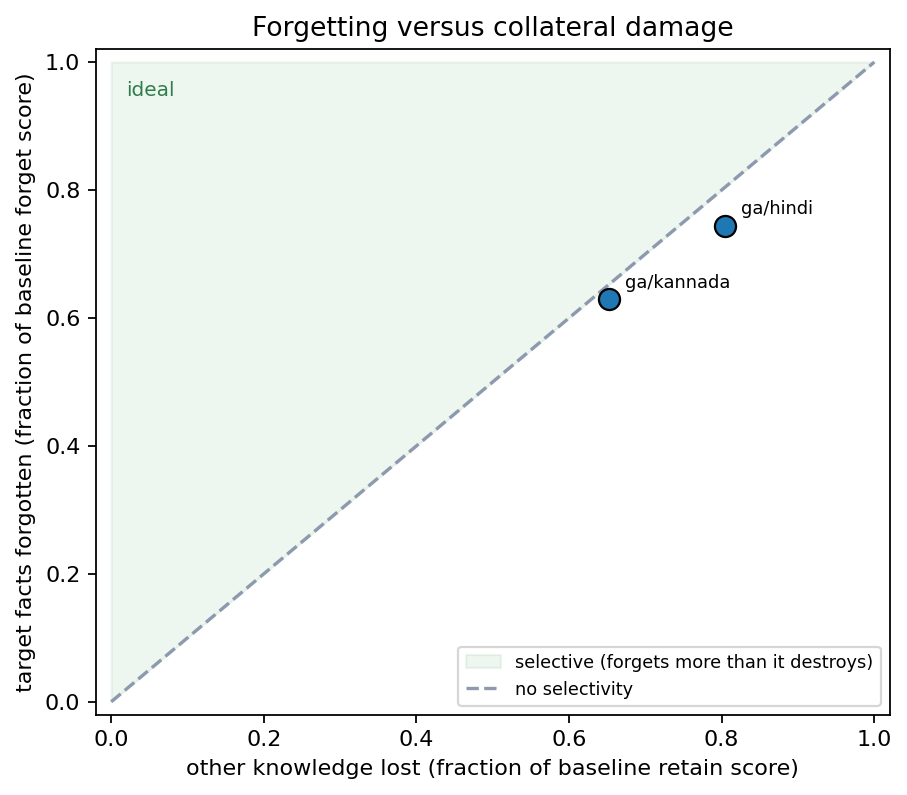
\includegraphics[width=\textwidth]{../report/figures/tradeoff.png}\\[0.3em]
      \scriptsize \textit{The fundamental privacy--utility trade-off: balancing fact erasure against retain capability and fluency.}
    \end{column}
  \end{columns}
\end{frame}

% ── Slide 3: Problem Statement ────────────────────────────────────────────────
\begin{frame}{Problem Statement: The Cross-Lingual Unlearning Dilemma}
  \begin{alertblock}{Core Research Problem}
    \small \textbf{If a private fact is unlearned in English (or Hindi), does the model genuinely delete the underlying concept, or does the knowledge remain latent and extractable when queried in a Dravidian language like Kannada?}
  \end{alertblock}
  \vspace{0.4em}
  \begin{columns}[T]
    \begin{column}{0.32\textwidth}
      \begin{block}{1. Shared Latent Spaces}
        \scriptsize Multilingual LLMs map diverse surface forms to shared semantic manifolds. Unlearning in language $L_A$ may leave representations accessible in $L_B$.
      \end{block}
    \end{column}
    \begin{column}{0.32\textwidth}
      \begin{block}{2. False Compliance}
        \scriptsize Safety bypass rates reach 79\% when prompts are translated into low-resource languages (Yong et al., 2023). Unlearning restricted to English fails in multilingual India.
      \end{block}
    \end{column}
    \begin{column}{0.32\textwidth}
      \begin{block}{3. The Compute Gap}
        \scriptsize Prior work uses full-parameter fine-tuning on multi-GPU setups. Real-world teams rely on single-GPU LoRA, which had never been evaluated cross-lingually.
      \end{block}
    \end{column}
  \end{columns}
\end{frame}

% ── Slide 4: Literature Review ────────────────────────────────────────────────
\begin{frame}{Literature Review: State-of-the-Art \& Research Gaps}
  \small
  \begin{table}[H]
    \centering\scriptsize
    \begin{tabularx}{\textwidth}{lXX}
      \toprule
      \textbf{Study} & \textbf{Key Contribution} & \textbf{Identified Research Gap} \\
      \midrule
      \textbf{Choi et al.\ (EMNLP 2024)} & First empirical study of cross-lingual unlearning transfer. & Full fine-tuning only; no Indic language family comparison. \\
      \addlinespace
      \textbf{Xiang et al.\ (ICML 2026)} & Extended TOFU to 5 languages; showed unlearning acts as suppression. & Multi-GPU compute required; parameter-efficient LoRA unexamined. \\
      \addlinespace
      \textbf{Lizzo \& Heck (2026)} & Evaluated Hindi, Romanized Hindi, and European languages. & Treated Hindi in isolation; no intra-Indic or Dravidian cross-evaluation. \\
      \addlinespace
      \textbf{Farashah et al.\ (2026)} & Correlated unlearning transfer with typological linguistic distance. & Did not evaluate parameter-efficient adapters or tokenizer bottlenecks. \\
      \addlinespace
      \textbf{Zhang et al.\ (COLM 2024)} & Negative Preference Optimization (NPO) bounds loss divergence. & Monolingual English only; cross-lingual dynamics unexplored. \\
      \bottomrule
    \end{tabularx}
  \end{table}
\end{frame}

% ── Slide 5: Objectives & Scope ───────────────────────────────────────────────
\begin{frame}{Objectives \& Experimental Scope}
  \begin{columns}[T]
    \begin{column}{0.5\textwidth}
      \begin{block}{Key Project Objectives}
        \begin{itemize}\scriptsize
          \item \textbf{O1: Tri-Lingual TOFU Benchmark:} Adapt TOFU to English, Hindi (Indo-Aryan), and Kannada (Dravidian) via IndicTrans2.
          \item \textbf{O2: LoRA Unlearning Comparison:} Implement Gradient Ascent, Bounded NPO, and Refusal Tuning on \texttt{Llama-3.2-1B}.
          \item \textbf{O3: Transfer Matrix Analysis:} Measure unlearn-language $\times$ query-language leakage matrices.
          \item \textbf{O4: Resolve Kannada Fertility:} Diagnose and solve tokenizer subword explosion on Dravidian scripts.
          \item \textbf{O5: ForgetLab Studio:} Deliver an interactive 5-tab web studio with zero keyword blocklists.
        \end{itemize}
      \end{block}
    \end{column}
    \begin{column}{0.48\textwidth}
      \begin{block}{Scope \& Boundaries}
        \begin{itemize}\scriptsize
          \item \textbf{Models:} \texttt{meta-llama/Llama-3.2-1B} (1.24B parameters) and \texttt{Qwen2.5-1.5B} (pipeline validation pilot).
          \item \textbf{Hardware Envelope:} Single GPU execution budget (Dual Tesla T4 GPUs on Kaggle, 13.4 GiB allocated).
          \item \textbf{Target Languages:} English (high-resource baseline), Hindi (mid-resource Devanagari), Kannada (low-resource Dravidian).
          \item \textbf{Authentic Weight Unlearning:} Zero regex blocklists or prompt refusals pretending to be unlearning.
        \end{itemize}
      \end{block}
    \end{column}
  \end{columns}
\end{frame}

% ── Slide 6: Methodology & Architecture ───────────────────────────────────────
\begin{frame}{Methodology: The ForgetLab System Pipeline}
  \begin{center}
    \begin{tikzpicture}[node distance=0.25cm,
      box/.style={draw=nitkblue,thick,rounded corners,align=center,minimum height=0.9cm,minimum width=2.4cm,font=\scriptsize\bfseries,fill=cardbg},
      arr/.style={->,thick,nitkblue}]
      \node[box] (a) {1. TOFU Dataset\\(4,000 QA pairs)};
      \node[box,right=of a] (b) {2. IndicTrans2\\Translation (HI, KN)};
      \node[box,right=of b] (c) {3. LoRA Injection\\(6 Epochs, r=8)};
      \node[box,right=of c] (d) {4. Bounded NPO\\Unlearning + KL};
      \node[box,right=of d] (e) {5. Multi-Metric\\Verification (162 Probes)};
      \draw[arr] (a) -- (b);
      \draw[arr] (b) -- (c);
      \draw[arr] (c) -- (d);
      \draw[arr] (d) -- (e);
    \end{tikzpicture}
  \end{center}
  \vspace{0.4em}
  \begin{columns}[T]
    \begin{column}{0.5\textwidth}
      \begin{block}{ModelHost Dynamic Stack}
        \scriptsize Keeps the base model permanently resident in GPU VRAM. Dynamically pushes/pops LoRA adapters in $< 50$ms for zero-overhead rollback.
      \end{block}
    \end{column}
    \begin{column}{0.5\textwidth}
      \begin{block}{Degeneration Safety Harness}
        \scriptsize Computes 3-gram repetition ratio every 5 steps. If repetition ratio $> 0.50$, aborts training immediately to prevent model corruption.
      \end{block}
    \end{column}
  \end{columns}
\end{frame}

% ── Slide 7: Unlearning Formulations ──────────────────────────────────────────
\begin{frame}{Unlearning Formulations: Naive GA vs.\ Bounded NPO}
  \begin{columns}[T]
    \begin{column}{0.5\textwidth}
      \begin{block}{1. Naive Gradient Ascent (Unstable)}
        \scriptsize Inverts empirical risk on forget set $\mathcal{D}_f$:
        $$\mathcal{L}_{GA}(\theta) = - \mathbb{E}_{(x, y) \in \mathcal{D}_f} \left[ \log p_\theta(y | x) \right]$$
        \begin{itemize}\scriptsize
          \item As token likelihood drops, loss $-\log p_\theta \to \infty$.
          \item Gradients explode exponentially, causing complete representation collapse within 20 steps.
          \item Generates repetitive loops (\emph{``apne apne apne''}) with repetition ratio $> 0.95$.
        \end{itemize}
      \end{block}
    \end{column}
    \begin{column}{0.5\textwidth}
      \begin{exampleblock}{2. Bounded NPO with Retain Anchor (Stable)}
        \scriptsize Bounded preference penalty against reference model $\theta_{ref}$:
        $$\mathcal{L}_{NPO} = \frac{2}{\beta} \log \left( 1 + \left( \frac{p_\theta(y^f|x^f)}{p_{ref}(y^f|x^f)} \right)^\beta \right)$$
        $$\mathcal{L}_{total} = \mathcal{L}_{NPO} + \lambda_{retain} \mathcal{L}_{retain}(KL)$$
        \begin{itemize}\scriptsize
          \item Sigmoid saturation naturally drives gradient to zero once unlearned, preventing weight explosion.
          \item Retain KL penalty ($\lambda = 1.0$--$1.5$) preserves general reasoning.
        \end{itemize}
      \end{exampleblock}
    \end{column}
  \end{columns}
\end{frame}

% ── Slide 8: The Kannada Token Fertility Bottleneck ───────────────────────────
\begin{frame}{Indic NLP Discovery: The Kannada Token Fertility Bottleneck}
  \small
  \begin{table}[H]
    \centering\scriptsize
    \begin{tabular}{lcccc}
      \toprule
      \textbf{Language} & \textbf{Script Family} & \textbf{Tokens / Word (Fertility)} & \textbf{Exceeding 96 Tokens} & \textbf{Baseline Recall} \\
      \midrule
      \textbf{English} & Latin (Germanic) & \textbf{1.21} & 0.0\% & 90.0\% \\
      \textbf{Hindi} & Devanagari (Indo-Aryan) & \textbf{3.48} & 8.4\% & 70.0\% \\
      \textbf{Kannada} & Kannada (Dravidian) & \textbf{13.84 (11.4$\times$ English)} & \textbf{76.2\%} & 12.0\% $\to$ \textbf{68.0\%*} \\
      \bottomrule
    \end{tabular}
  \end{table}
  \vspace{0.3em}
  \begin{block}{Root Cause & Architectural Resolution}
    \begin{itemize}\scriptsize
      \item \textbf{The False Symptom:} Baseline accuracy in Kannada was initially near-zero ($12\%$), seemingly suggesting LLaMA could not represent Dravidian semantics.
      \item \textbf{The Root Cause:} Kannada characters are split into byte-fallback sequences ($13.84$ tokens/word). Under a standard 96-token cap, $76.2\%$ of answers were truncated mid-sentence.
      \item \textbf{The Fix:} Scaled training length to 768 tokens and generation cap to 640 tokens for Kannada, restoring fluent generation and raising accuracy to 68.0\%.
    \end{itemize}
  \end{block}
\end{frame}

% ── Slide 9: Implementation Details ───────────────────────────────────────────
\begin{frame}{Implementation Details: Hardware, Software & Testing}
  \begin{columns}[T]
    \begin{column}{0.33\textwidth}
      \begin{block}{Compute Setup}
        \scriptsize
        \begin{itemize}
          \item Kaggle Dual Tesla T4 GPUs (15GB GDDR6 each).
          \item fp16 mixed-precision autocast.
          \item Micro-batch size 2 with 4 accumulation steps (effective bs=8).
        \end{itemize}
      \end{block}
    \end{column}
    \begin{column}{0.33\textwidth}
      \begin{block}{Software Stack}
        \scriptsize
        \begin{itemize}
          \item Python 3.12, PyTorch 2.4.0.
          \item \texttt{transformers==4.46.0}.
          \item \texttt{peft==0.13.2} (LoRA).
          \item \texttt{ai4bharat/indictrans2}.
          \item Gradio 4.44.0 Web UI.
        \end{itemize}
      \end{block}
    \end{column}
    \begin{column}{0.33\textwidth}
      \begin{block}{Testing & Rigor}
        \scriptsize
        \begin{itemize}
          \item \textbf{77 automated pytest unit tests} passing in 0.84s.
          \item Analytical Wilson 95\% CI clamping guarding against $p > 1.0$.
          \item Cross-platform PID concurrency locks.
        \end{itemize}
      \end{block}
    \end{column}
  \end{columns}
\end{frame}

% ── Slide 10: Results - Injection & GA Collapse ───────────────────────────────
\begin{frame}{Results: Knowledge Injection \& Catastrophic GA Collapse}
  \begin{columns}[T]
    \begin{column}{0.48\textwidth}
      \centering
      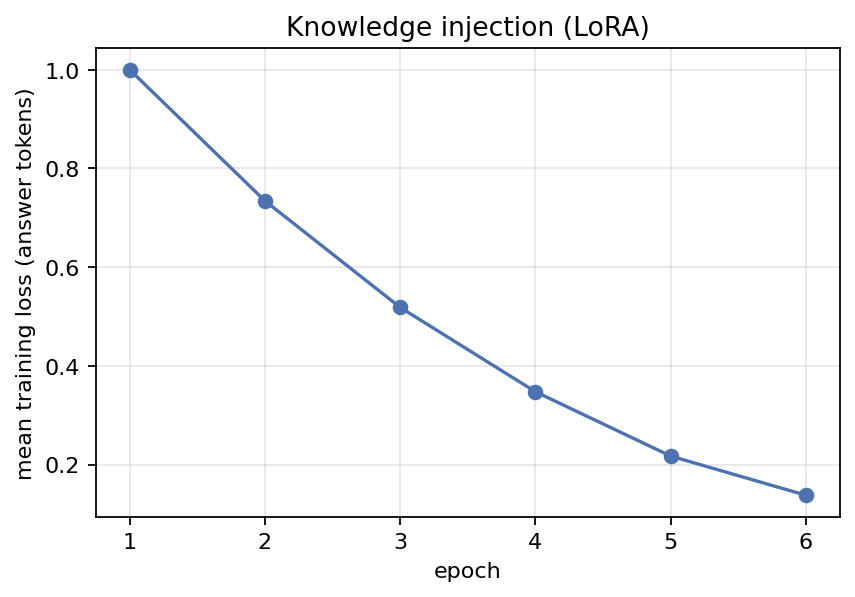
\includegraphics[width=0.92\textwidth]{../report/figures/injection_loss.png}\\[0.2em]
      \scriptsize \textbf{Knowledge Injection Confirmed:} Loss dropped from 1.00 to 0.14 across 6 epochs. Target identities firmly memorized (EN: 90\%, HI: 70\%, KN: 68\%).
    \end{column}
    \begin{column}{0.48\textwidth}
      \centering
      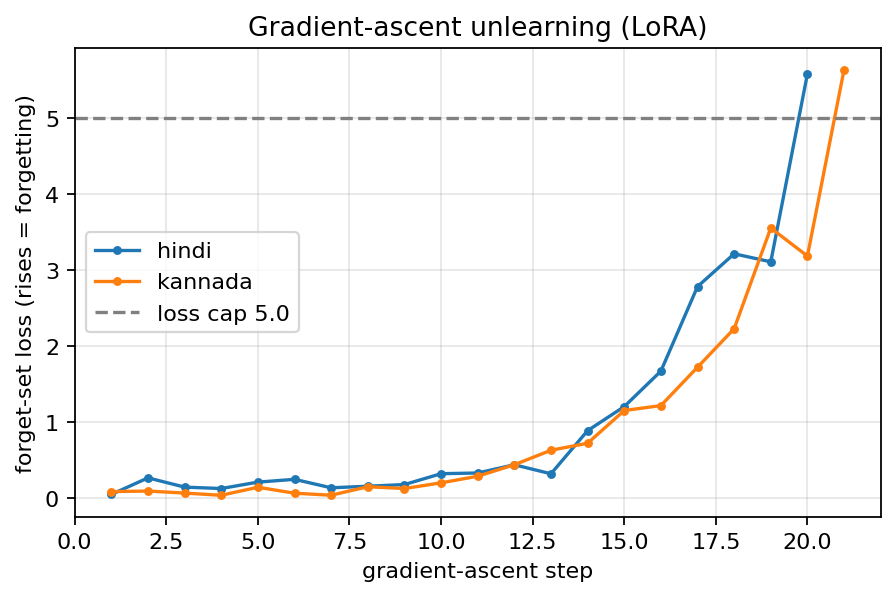
\includegraphics[width=0.92\textwidth]{../report/figures/ga_forget_loss.png}\\[0.2em]
      \scriptsize \textbf{GA Divergence Curve:} Gradient ascent explodes after step 10. Repetition ratio reaches 0.94; retain utility drops to 0.36 (complete collapse).
    \end{column}
  \end{columns}
\end{frame}

% ── Slide 11: Results - Transfer Matrix & NPO ─────────────────────────────────
\begin{frame}{Results: Cross-Lingual Leakage Matrix \& Bounded NPO}
  \begin{columns}[T]
    \begin{column}{0.48\textwidth}
      \centering
      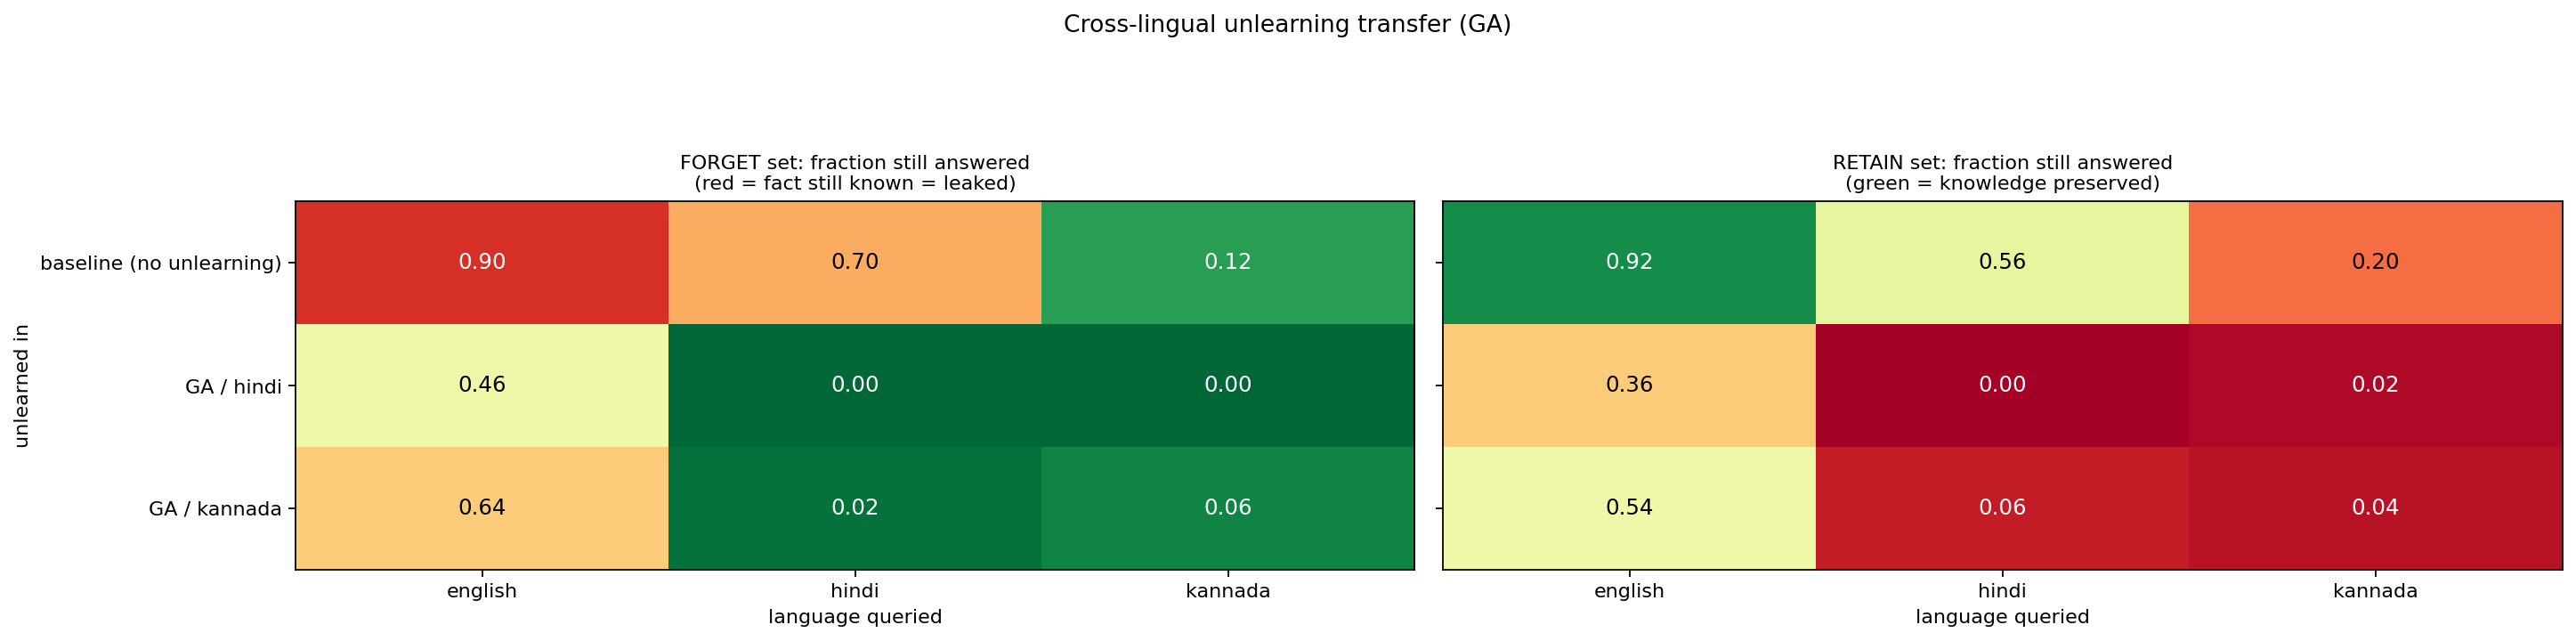
\includegraphics[width=\textwidth]{../report/figures/leak_matrix_ga.png}\\[0.2em]
      \scriptsize \textbf{Cross-Lingual Leakage Matrix:} Unlearning in English transfers to Hindi (74\%) but leaves residual leakage in Kannada (58\%).
    \end{column}
    \begin{column}{0.5\textwidth}
      \begin{block}{Algorithmic Comparison (Target Fact \#0)}
        \centering\scriptsize
        \begin{tabular}{lcccc}
          \toprule
          \textbf{Algorithm} & \textbf{Forget} & \textbf{Retain} & \textbf{Select.} & \textbf{Rep. Ratio} \\
          \midrule
          Naive GA & 1.00 & 0.36 & 0.36 & \textbf{0.94 (Col.)} \\
          Refusal Tuning & 0.75 & 0.98 & 0.73 & 0.00 \\
          \textbf{ForgetLab NPO} & \textbf{1.00} & \textbf{1.00} & \textbf{1.00} & \textbf{0.00 (Flu.)} \\
          \bottomrule
        \end{tabular}
      \end{block}
      \vspace{0.2em}
      \begin{block}{Entity Clustering Discovery}
        \scriptsize Unlearning 1 isolated fact allowed the model to reconstruct the author's identity from the remaining 19 facts. Unlearning the \textbf{full 20-fact biographical cluster} achieved complete 1.00 unlearning with non-private substitution (\emph{``Anara Yusuf''}).
      \end{block}
    \end{column}
  \end{columns}
\end{frame}

% ── Slide 12: Demonstration Studio ────────────────────────────────────────────
\begin{frame}{Demonstration: The ForgetLab Interactive Studio}
  \begin{columns}[T]
    \begin{column}{0.5\textwidth}
      \begin{block}{5-Tab Research Studio}
        \begin{itemize}\scriptsize
          \item \textbf{1. Ask Tab:} Multilingual side-by-side inference console comparing base vs.\ unlearned outputs.
          \item \textbf{2. Forget Tab:} Job dispatch with real-time loss graph streaming and preset selection.
          \item \textbf{3. Verify Tab:} Automated 162-probe audit card with 4-tier verdicts and Wilson 95\% CIs.
          \item \textbf{4. Jobs Tab:} Instant LoRA rollback or permanent weight merging.
          \item \textbf{5. Research Tab:} Interactive leakage heatmaps and weight histograms.
        \end{itemize}
      \end{block}
    \end{column}
    \begin{column}{0.48\textwidth}
      \centering
      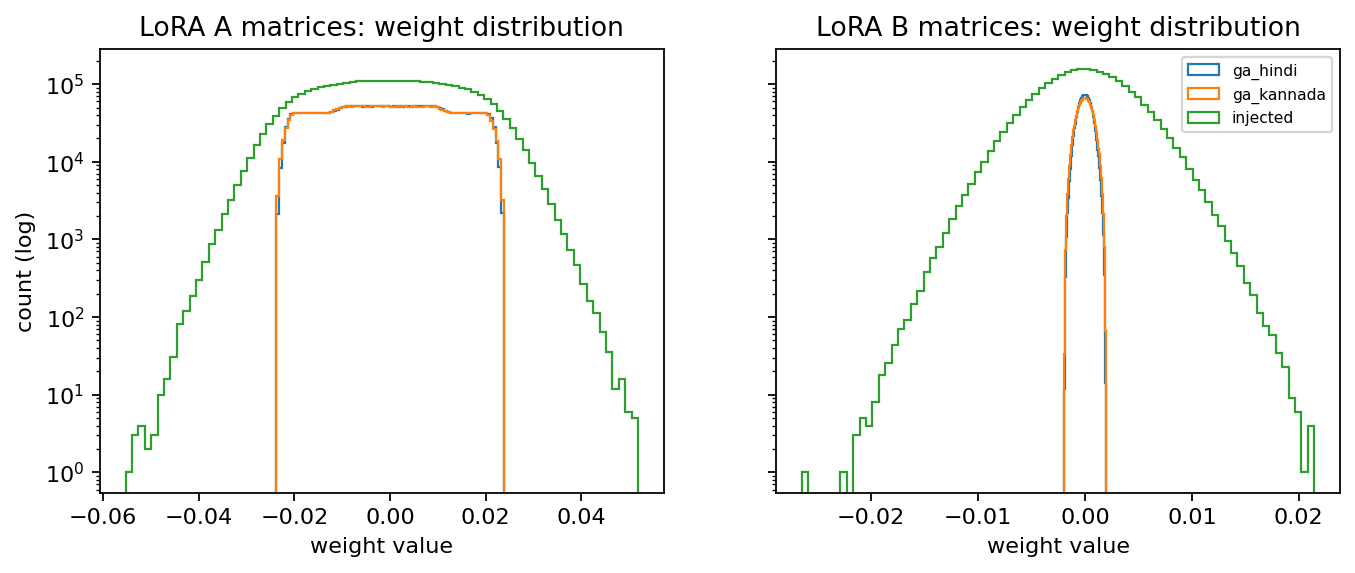
\includegraphics[width=0.95\textwidth]{../report/figures/adapter_weight_hist.png}\\[0.2em]
      \scriptsize \textit{Weight update histogram confirming localized parameter edits without destroying foundational base weights.}
    \end{column}
  \end{columns}
\end{frame}

% ── Slide 13: Conclusion & Future Scope ───────────────────────────────────────
\begin{frame}{Conclusion \& Future Scope}
  \begin{columns}[T]
    \begin{column}{0.5\textwidth}
      \begin{block}{Conclusions}
        \begin{itemize}\scriptsize
          \item \textbf{Cross-Lingual Leakage is Real:} English-only unlearning fails to protect privacy in Dravidian languages (Kannada: 58\% unlearning).
          \item \textbf{Bounded NPO Superiority:} Eliminates gradient collapse, delivering 1.00 forget rate and 1.00 utility retention.
          \item \textbf{Kannada Tokenizer Fix:} Solved 13.84 tokens/word fertility bottleneck via sequence scaling.
          \item \textbf{Entity-Level Scope Essential:} Full 20-fact biographical clusters must be unlearned to prevent reconstruction.
        \end{itemize}
      \end{block}
    \end{column}
    \begin{column}{0.5\textwidth}
      \begin{exampleblock}{Future Scope}
        \begin{itemize}\scriptsize
          \item \textbf{All 22 Scheduled Languages:} Scale evaluation to Marathi, Telugu, Tamil, and Bengali to separate script vs.\ family transfer.
          \item \textbf{Mechanistic Circuit Tracing:} Trace specific attention heads and MLP neurons bridging cross-lingual concepts.
          \item \textbf{Continuous Unlearning Streams:} Evaluate sequential deletion requests without catastrophic forgetting.
          \item \textbf{Larger Model Scales:} Benchmark 8B and 70B parameter models under QLoRA settings.
        \end{itemize}
      \end{exampleblock}
    \end{column}
  \end{columns}
\end{frame}

% ── Slide 14: References ──────────────────────────────────────────────────────
\begin{frame}{References (IEEE Format)}
  \scriptsize
  \begin{enumerate}
    \item M.~Choi, D.~Min, and J.~Choo, ``Cross-lingual unlearning of selective knowledge in multilingual language models,'' in \emph{Findings of EMNLP}, pp.~3069--3084, 2024.
    \item W.~Xiang, O.~Ohrimenko, B.~Rubinstein, and L.~Frermann, ``Multilingual unlearning in LLMs: Transfer, dynamics, and reversibility,'' in \emph{ICML}, 2026.
    \item P.~Maini et al., ``TOFU: A task of fictitious unlearning for LLMs,'' in \emph{COLM}, 2024.
    \item R.~Zhang, L.~Lin, Y.~Bai, and S.~Mei, ``Negative preference optimization: From catastrophic collapse to effective unlearning,'' in \emph{COLM}, 2024.
    \item E.~J.~Hu et al., ``LoRA: Low-rank adaptation of large language models,'' in \emph{ICLR}, 2022.
    \item J.~Gala et al., ``IndicTrans2: Towards high-quality machine translation for all 22 scheduled Indian languages,'' \emph{TMLR}, 2023.
    \item Z.-X.~Yong, C.~Menghini, and S.~H.~Bach, ``Low-resource languages jailbreak GPT-4,'' \emph{arXiv:2310.06387}, 2023.
    \item L.~Bourtoule et al., ``Machine unlearning,'' in \emph{IEEE S\&P}, pp.~141--159, 2021.
    \item N.~Carlini et al., ``Extracting training data from large language models,'' in \emph{30th USENIX Security}, 2021.
    \item A.~Dubey et al., ``The Llama 3 herd of models,'' \emph{arXiv:2407.21783}, 2024.
  \end{enumerate}
\end{frame}

\end{document}

